\chapter{Analyzing the genetic structure of populations: individual assignment}

Although $F$-statistics are widely used and very informative, they
suffer from one fundamental limitation: We have to know what the
populations are before we can estimate them.\footnote{To be a little
  more precise~(and more than a little pedantic), we have to {\it
    assume\/} that the sample locations we decide to treat as
  populations are discrete, well-mixed populations that are distinct
  from others.} They are based on a conceptual model in which
organisms occur in discrete populations, populations that are both (1)
well mixed within themselves (so that we can regard our sample of
individuals as a random sample from within each population) and (2)
clearly distinct from others. What if we want to use the genetic data
itself to help us figure out what the populations actually are? Can we
do that?\footnote{Would I be asking this question if the answer were
  ``No?''}

A little over 20 years ago a different approach to the analysis of
genetic structure began to emerge: analysis of individual
assignment.\index{individual assignment} Although the implementation
details get a little hairy,\footnote{OK, to be fair. They get {\it
    very\/} hairy.} the basic idea is fairly simple. I'll give an
outline of the math in a moment, but let's do this in words
first. Suppose we have data on a series of individuals. If two
individuals are part of the same population, we expect them to be more
similar to one another than they are to individuals in other
populations. So if we ``cluster'' individuals that are ``genetically
similar'' to one another, those clusters should correspond to
populations. Rather than pre-defining the populations, we will have
allowed the data to tell us what the populations are. We haven't even
required {\it a priori\/} that individuals be grouped according to
their geographic proximity. Instead, we can examine the clusters we
find and see if they make any sense geographically.

Now for an outline of the math. Label the data we have for each
individual $x_i$. Suppose that all individuals belong to one of $K$
populations\footnote{Remember the peculiar thing I mentioned about
  population geneticists earlier? We like to imagine we know something
  even when we don't. In this case, I'm imagining we know that there
  are $K$ even though we don't. If we knew $K$, we'd probably already
  know which individual belonged in which population. We'll get to the
  problem of determining what $K$ is later.} and let the genotype
frequencies in population $k$ be represented by $\gamma_k$. Then the
likelihood that individual $i$ comes from population $k$ is just
\[
\mbox{P}(i|k) = \frac{\mbox{P}(x_i|\gamma_k)}{\sum_k
  \mbox{P}(x_i|\gamma_k)} \quad .
\]
So if we can specify prior probabilities for $\gamma_k$, we can use
Bayesian methods to estimate the posterior probability that individual
$i$ belongs to population $k$, and we can associate that assignment
with some measure of its reliability.\footnote{You can find details
  in~\cite{Pritchard-etal-2000}. If you think about that equation a
  bit, you can begin to see why the details get {\it very\/}
  hairy. First, we're trying to get the data to tell us what the
  populations are, so we don't even know how many populations there
  are. Then we have to find a way of estimating allele frequencies
  (and genotype frequencies) in populations when we don't even know
  which populations individuals in our sample belong in.}  Remember,
though, that we've arrived at the assignment by {\it assuming\/} that
there are $K$ populations. Since we don't know $K$, we have to find a
way of estimating it. Different choices of $K$ may lead to different
patterns of individual assignment, which complicates our
interpretation of the results.\footnote{This is an example of the ``no
  free lunch'' principle. You don't get something for nothing. Here we
  gained the ability to have the data tell us what the populations
  are, but we made interpreting the results more difficult.}

\section*{Applying assignment to understand invasions}

To see a simple example of how {\tt
  Structure}\index{Structure@\texttt{Structure}} can be used, we'll
use it to assess whether cultivated genotypes of {\it Berberis
  thunbergii\/}\index{Berberis@\textit{Berberis}!\textit{thunbergii}}
contribute to ongoing invasions in Connecticut and
Massachusetts~\cite{Lubell-etal-2008}.\index{individual assignment!application} The first problem is to determine what $K$
to use, because $K$ doesn't necessarily have to equal the number of
populations we sample from. Some populations may not be distinct from
one another. There are a couple of ways to estimate $K$. The most
straightforward is to run the analysis for a range of plausible
values, repeat it 10-20 times for each value, calculate the mean ``log
probability of the data'' for each value of $K$, and pick the value of
$K$ that is the biggest, i.e., the least
negative~(Table~\ref{table:berberis-k}). For the barberry data, $K=3$
is the obvious choice.\footnote{As part of her dissertation, Nora
  Mitchell used {\tt Structure} to study a hybrid zone between two
  species of {\it Protea}~\cite{Mitchell-Holsinger-2018}. Nora was
  interested in determining the extent to which individuals reflected
  ancestry from one of the two species involved. She set $K=2$ to
  separate individuals as cleanly into two categories as possible and
  used the individual assignment score as an index of hybridity. There
  wasn't any reason to attempt to infer $K$ from the data.}

\begin{table}
\begin{center}
\begin{tabular}{cc}
\hline\hline
K & Mean L(K) \\
\hline
2 & -2553.2 \\
3 & {\bf -2331.9} \\
4 & -2402.9 \\
5 & -2476.3 \\
\hline
\end{tabular}
\end{center}
\caption{Mean log probability of the data for $K=2,3,4,5$ in the {\it
    Berberis thunbergii\/} data~(adapted
  from~\cite{Lubell-etal-2008}).}\label{table:berberis-k}
\end{table}

Having determined that the data support $K=3$, the results of the
analysis are displayed in Figure~\ref{fig:lubell-structure}. Each
vertical bar corresponds to an individual in the sample, and the
proportion of each bar that is of a particular color tells us the
posterior probability that the individual belongs to the cluster with
that color.

\begin{figure}
\resizebox{\textwidth}{!}{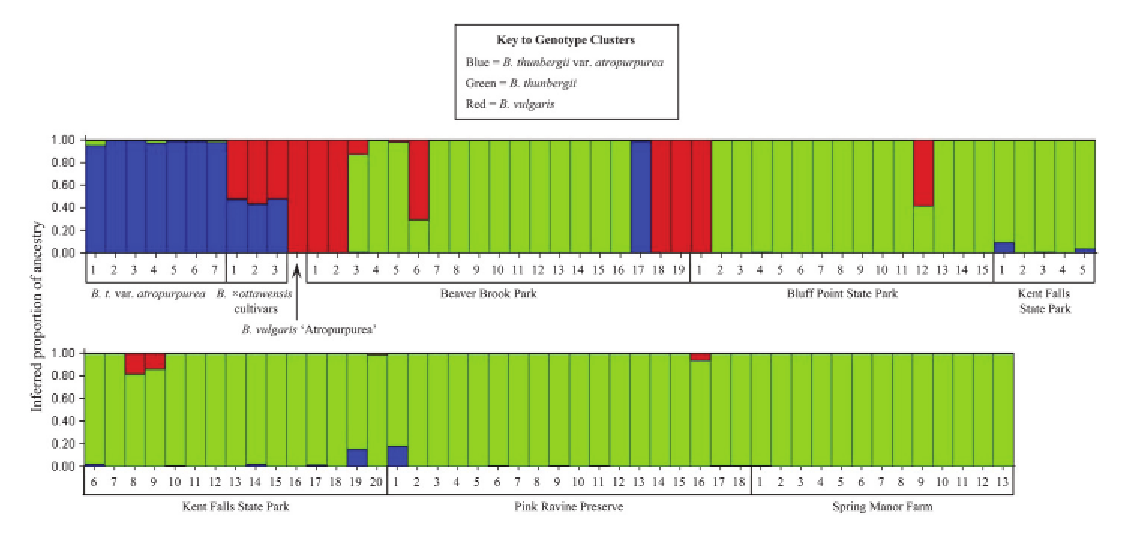
\includegraphics{lubell-structure.eps}}
\caption{Analysis of AFLP data from {\it Berberis
    thunbergii}~\cite{Lubell-etal-2008}.}\label{fig:lubell-structure} 
\end{figure}

Figure~\ref{fig:lubell-structure} may not look terribly informative,
but actually it is. Look at the labels beneath the figure. You'll see
that with the exception of individual 17 from Beaver Brook Park, all
the of the individuals that are solid blue are members of the
cultivated {\it Berberis thunbergii\/} var. {\it atropurpurea}. The
solid red bar corresponds to {\it Berberis vulgaris\/} 'Atropurpurea',
a different modern cultivar.\footnote{I find it very confusing that
  {\it Berberis thunbergii\/} var. {\it atropurpurea\/} and {\it
    Berberis vulgaris\/} 'Atropurpurea' both have ``atropurpurea''
  associated with their names, but that's the way life is.} You'll
notice that individuals 1, 2, 18, and 19 from Beaver Brook Park and
individual 1 from Bluff Point State Park fall into the same genotypic
cluster as this cultivar. {\it Berberis $\times$ottawensis} is a
hybrid cultivar whose parents are {\it Berberis thunbergii\/} and {\it
  Berberis vulgaris\/}, so it makes sense that individuals of this
cultivar would be half blue and half red. The solid green bars are
feral individuals from long-established populations. Notice that the
cultivars are distinct from all but a few of the individuals in the
long-established feral populations, suggesting that contemporary
cultivars are doing relatively little to maintain the invasion in
areas where it is already established.

\section*{Genetic diversity in human populations}\index{humans}

A much more interesting application of {\tt Structure} appeared a
shortly after {\tt Structure} was introduced. The Human Genome
Diversity Cell Line Panel (HGDP-CEPH)\index{HGDP-CEPH} consisted at
the time of data from 1056 individuals in 52 geographic
populations. Each individual was genotyped at 377 autosomal loci. If
those populations are grouped into 5 broad geographical
regions~(Africa, [Europe, the Middle East, and Central/South Asia],
East Asia, Oceania, and the Americas), we find that about 93\% of
genetic variation is found within local populations and only about 4\%
is a result of allele frequency differences between
regions~\cite{Rosenberg-etal-2002}. You might wonder why Europe, the
Middle East, and Central/South Asia were grouped together for that
analysis. The reason becomes clearer when you look at a {\tt
  Structure} analysis of the data~(Figure~\ref{fig:HGDP-CEPH}).

\begin{figure}
\resizebox{\textwidth}{!}{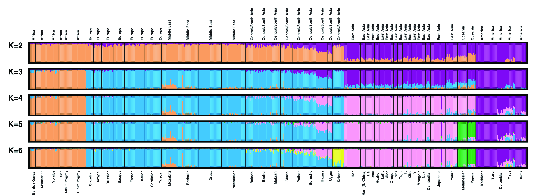
\includegraphics{HGDP-CEPH.eps}}
\caption{{\tt Structure} analysis of microsatellite diversity in the
  Human Genome Diversity Cell Line
  Panel~(from~\cite{Rosenberg-etal-2002}).}\label{fig:HGDP-CEPH} 
\end{figure}

\subsection*{A non-Bayesian look at individual-based analysis of
  genetic structure}

{\tt Structure} has a lot of nice features, but you'll discover a
couple of things about it if you begin to use it seriously: (1) It
often isn't obvious what the ``right'' {\tt K} is.\footnote{In fact,
  it's not clear that there {\it is\/} such a thing as the ``right''
  {\tt K}. If you're interested in hearing more about that. Feel free
  to ask.} (2) It requires a {\it lot\/} of computational resources,
especially with datasets that include a few thousand SNPs, as is
becoming increasingly common. An alternative is to use principal
component analysis directly on genotypes. There are technical details
associated with estimating the principal components and interpreting
them that we won't discuss,\footnote{See~\cite{Novembre-Stephens-2008}
  for details}, but the results can be pretty
striking. Figure~\ref{fig:human-PCA} shows the results of a PCA on
data derived from 3192 Europeans at 500,568 SNP loci. The
correspondence between the position of individuals in PCA space and
geographical space is remarkable. 

\begin{figure}
\resizebox{\textwidth}{!}{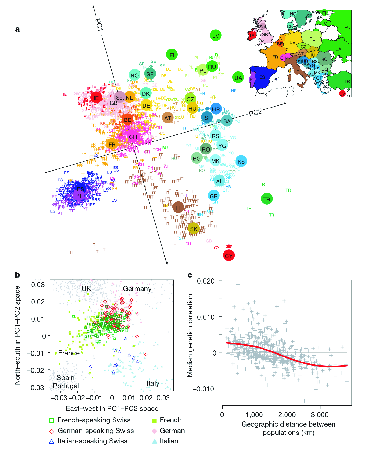
\includegraphics{human-PCA.eps}}
\caption{Principal components analysis of genetic diversity in Europe
  corresponds with
  geography~(from~\cite{Novembre-etal-2008}). Panel b is a close-up
  view of the area around Switzerland~(CH).}\label{fig:human-PCA}
\end{figure}

\section*{Other approaches}

Jombart et al.~\cite{Jombart-etal-2010} describe a related method
known as discriminant analysis of principal components. They also
provide an {\tt R} package, {\tt dapc}, that implements the
method.\index{Discriminant analysis of population structure} I prefer
{\tt Structure} because its approach to individual assignment is based
directly on population genetic principles, and since computers are
getting so fast~(especially when you have a computational cluster
available) that I worry less about how long it takes to run an
analysis on large datasets.\footnote{I also remember that a very long
  time ago when systematists were complaining that likelihood analyses
  of their data sets were taking a couple of weeks, Joe Felsenstein
  was reported to have said ``Why are you complaining that your
  analysis is taking a couple of weeks when you spent a couple of
  years collecting the data?''} That being said, Gopalan et
al.~\cite{Gopalan-etal-2016} released {\tt teraStructure} about five
years ago, which can analyze data sets consisting of 10,000
individuals scored at a million SNPs in less than 10
hours.\index{teraStructure@\texttt{teraStructure}} I haven't tried it
myself, because I haven't had a large data set to try it on, but you
should keep it in mind if you collect SNP data on a large number of
loci. Here are a couple more alternatives to consider that I haven't
investigated yet:

\begin{itemize}

\item {\tt sNMF} estimates individual admixture coefficients. It is
  reportedly 10-30 faster than the likelihood based {\tt ADMIXTURE},
  which is itself faster than {\tt Structure}. {\tt sNMF} is part of
  the {\tt R} package {\tt LEA}.

\item Meisner and Albrecthsen~\cite{Meisner-Albrechtsen-2018} present
  both a principal components method and an admixture method that
  accounts for sequencing errors inherent in low-coverage next
  generation DNA sequencing data.

\end{itemize}

